% use UTF-8 encoding in editors such as TeXworks
% !TEX encoding = UTF-8 Unicode
% !TEX TS-program = pdflatex

\documentclass[%
    corpo=13.5pt,
    twoside,
%    stile=classica,
    oldstyle,
%    autoretitolo,
    tipotesi=magistrale,
    greek,
    evenboxes
]{toptesi}

\usepackage[utf8]{inputenc}% codifica d'entrata
\usepackage[T1]{fontenc}%    codifica dei font
\usepackage{lmodern}%        scelta dei font
\usepackage{listings}       % code listing
\usepackage{mathtools}      % math
\usepackage{url}            % URLs usage: \url{https://example.com}
\usepackage{cite}           % cite bibtex entries

% Vedere la documentazione toptesi-it.pdf per le
% attenzioni che bisogna usare al fine di ottenere un file
% veramente conforme alle norme per l'archiviabilità.

\usepackage{hyperref}
\hypersetup{%
    pdfpagemode={UseOutlines},
    bookmarksopen,
    pdfstartview={FitH},
    colorlinks,
    linkcolor={blue},
    citecolor={blue},
    urlcolor={blue}
  }

%%%%%%% Definizioni locali
\newtheorem{osservazione}{Osservazione}% Standard LaTeX
\ExtendCaptions{english}{Abstract}{Acknowledgements}



\begin{document}\errorcontextlines=9

% set english ad primary language
\english

%%%%%%%%%%%%%%%%%%%%
% BEGIN front page %
%%%%%%%%%%%%%%%%%%%%
\begin{ThesisTitlePage}*

\ateneo{Politecnico di Torino}
\nomeateneo{DEPARTMENT OF CONTROL AND COMPUTER ENGINEERING}
\CorsoDiLaureaIn{Master of Science in}
\corsodilaurea{Computer Engineering}
\TesiDiLaurea{Master Degree Thesis}

\titolo{Deep Learning on Polito Knowledge Graph}
\sottotitolo{Leveraging Relational GCN for link prediction between nodes of a newly built publications graph}

\CandidateName{Candidate}
\candidato{Giovanni \textsc{Garifo}}

\AdvisorName{Supervisors}
\relatore{Prof.~Antonio Vetrò}
\secondorelatore{Prof.~Juan Carlos De Martin}
\sedutadilaurea{\textsc{Academic~Year} 2018-2019}%

\logosede[6cm]{logopolito}
\end{ThesisTitlePage}
%%%%%%%%%%%%%%%%%%
% END front page %
%%%%%%%%%%%%%%%%%%


% offset rilegatura
%\setbindingcorrection{3mm}

\makeatletter
\newenvironment{miadedica}{
    \clearpage
    \if@twoside
        \ifodd\c@page\else\thispagestyle{empty}\null\clearpage\fi
    \fi
    \thispagestyle{empty}%
    \list{}{\labelwidth\z@
    \leftmargin.73\textwidth
    \parindent\z@
    \raggedright\LARGE\itshape}\item[]
    \normalsize
}

\begin{miadedica}
    To Monia\\
    To my Grandfather
\end{miadedica}


\paginavuota
\sommario

Summary here, one page


\ringraziamenti

Acknowledgements here, half page


\tablespagetrue\figurespagetrue % normalmente questa riga non serve ed e' commentata
\indici

\mainmatter

\chapter{Introduction}

\section{Motivation}

Graphs are used to empower some of the most complex IT services available
today, an example among all being the Google search engine
\footnote{\url{https://blog.google/products/search/introducing-knowledge-graph-things-not/}}.
They can be used to represent almost any kind of information, and they are
particurlarly capable of representing the structure of complex systems and
describe the relationships between their elements.

Over the last decade, much effort has been made in trying to leverage the power
of graphs to represent human knowledge and to build search tools capable of
querying and understanding the semantic relations within them. RDF graphs are a
particular class of graphs that can be used to build knowledge
repositories. Given a domain and an ontology, they allows to build a structured
representation of the knowledge in such domain.

Modern machine learning techniques can be used to mine latent information
from such graphs. One of the main challenges in this field is how to learn
meaningful representations of entities and relations that embed
the underlying knowledge. Such representations can then be used to evaluate
new links inside the graph or to classify unseen nodes.
Deep learning techniques have proved to be first class citizens when
dealing with representation learning tasks, being able to learn latent
representations without any prior knowledge other than the graph structure,
so as not to require any feature engineering.



\section{Thesis structure}

\subsection{Chapter 2}

\subsection{Chapter 3}

\subsection{Chapter 4}



\chapter{Background}

\section{Semantic Web}

\subsection{From a Web of contents to a Web of data}

The World Wide Web has been developed as a tool to easily access
documents and to navigate through them by following hyperlinks.
This simple description already resembles the structure of a graph: we can
think of documents as nodes, and of hyperlinks as edges. The unstoppable growth
of the \emph{Web graph} led to the emergence of new tools to extricate in such
complexity. Search engines have been developed to easily navigate such a giant
graph, initially by scoring search results based on trivial statistics, such
as the number of times a document has been linked, as in the case of the
PageRank \cite{page1999} algorithm developed by Google.
\newline

The Web rapidly became one of the most innovative technology ever built,
allowing to retrive information quickly and easily as never before.
The next evolutionary step has been to think about a Web not only exploitable by
human beings but also by machines. In order to build such a comprehensive
system, where information can be not only machine-readable, but
machine-understandable, the World Wide Web had to move from a web of content, to
a web of data.
\newline

The World Wide Web Consortium (W3C) introduced the Semantic Web as an extention
to the prior standard of the WWW. Its primary goal has been
to define a framework to describe and query semantic information contained
in the documents available on the web, so as to allow machines to understand
the semantic information contained in web pages. In the vision of Tim
Berners-Lee, the father of WWW, this would bring to the transition from a
World Wide Web to a Giant Global Graph
\footnote{\url{https://web.archive.org/web/20160713021037/http://dig.csail.mit.edu/breadcrumbs/node/215}},
where a web page contains metadata that provides to a machine the needed
information to understand the concepts and meanings expressed in it.


\subsection{The Semantic Web building blocks}

The three key components of the Semantic Web standard are:
\begin{enumerate}
\item OWL: the Web Ontology Language
\item RDF: the Resource Description Framework
\item SPARQL: The SPARQL Protocol and RDF Query Language
\end{enumerate}
\bigskip

OWL is a language used to define ontologies. In this context, an ontology
is defined as a collection of concepts, relations and constraints between
these concepts that describes an area of interest or a domain.
OWL allows to classify things in terms of their meaning by describing
their belonging to classes and subclasses defined by the ontology: if
a thing is defined as member of a class, this means that it shares the
same semantic meaning as all the other members of such class. The result of
such classification is a taxonomy that defines a hierarchy of how things
are semantically interrelated in the domain under analysis.
The instances of OWL classes are called individuals, and can be related
with other individuals or classes by means of properties. Each individual
can be characterized with additional information using literals, that
represent data values like strings, dates or integers.
\newline

RDF is a XML-based framework that defines a standard model for the
description, modelling and interchange of resources on the Web.

The first component of the framework is the \emph{RDF Model and Syntax},
which defines a data model that describes how the RDF resources should be
represented. The basic model consist of only three object types: resource,
property, and statement.
A resource is uniquely identified by an Uniform Resource Identifier (URI).
A property can be both a resource attribute or a relation between resources.
A statement describes a resource property, and is defined as a triple
between a subject (the resource), a predicate (the property) and an
object (a literal or another resource).

The second component of the framework is the \emph{RDF Schema} (RDFS),
that defines a basic vocabulary for describing RDF resources and the
relationships between them. Many vocabularies have been built on top of
RDFS, such as the Friend of a Friend (FOAF) vocabulary \cite{brickley2007}, for
describing social networks, or the one maintained by the Dublin Core Metadata
Initiative \footnote{\url{https://www.dublincore.org/}}, that defines common
terms used in the definition of metadata for digital resources.

\begin{figure}[ht]
\centering
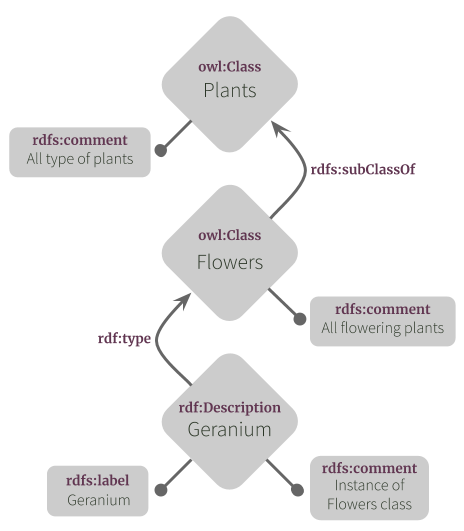
\includegraphics[scale=0.6]{img/owl-ontology-example.png}
\caption{An example of ontology defined using OWL and RDF Schema.}
\label{fig:owl-ontology-example}
\end{figure}

SPARQL is a query language for triplestores, a class of Database
Management Systems (DBMS) specialized in storing RDF databases. Such DBMS
often expose endpoints that can be used to query the database and obtain
results. Given the complexity of the data stored, the query language has
been designed to be as simple as possible, in example by allowing the use
of variables, whose definition is preceded by a question mark.

The syntax of SPARQL is heavily derived from SQL, with some
minor adaptations to be more suited for querying graphs data. The
following is an example of query which selects all the labels
(human-readable description of a resource) of all the entities that
matches the given resource type.

\begin{lstlisting}[
        language=sparql,
        frame=single,
    ]
    PREXIF plants:<http://example.org/plants/>

    SELECT ?name
    WHERE {
        ?subject rdf:type plants:flowers .
        ?subject rdfs:label ?name .
    }
\end{lstlisting}

\subsection{Knowledge Bases as knowledge repositories}

Even if the raise of the Semantic Web has suffered a slowdown in its growth
due to the complexity of its vision, many new projects were born from its
enabling technologies. Efforts have been put by profit and
non-profit organizations in trying to build complex knowledge repositories
starting from the knowledge already present in the Web. An example among all
is the DBpedia\footnote{\url{https://wiki.dbpedia.org/}} project, which
developed a structured knowledge base from the unstructured data available on
Wikipedia.
Another example is the
\emph{Google Knowledge Graph}\footnote{\url{https://blog.google/products/search/introducing-knowledge-graph-things-not/}},
which is used to enhance the Google search engine and virtual assistant
capabilities, allowing to retrieve punctual information about everything that
has been classified in its ontology and described in its knowledge base, or
the \emph{Open Academic Graph}\footnote{\url{https://www.openacademic.ai/oag/}},
a Scientific Knowledge Graph that contains, describes and links more then
three hundred million academic papers.

From an implementation perspective, knowledge bases can be created to
describe a specific domain by defining an ontology and a vocabulary for
such domain using OWL and RDF Schema, and then by describing the concepts
of such domain using the RDF Model and Syntax. The RDF document obtained
can then be stored in a triplestore and queryed using SPARQL. The biggest effort
when building knowledge bases is to have a correct understanding and prior
knowledge of the domain of interest, to avoid the risk of mischaracterizing
and misrepresenting concepts.

\begin{figure}[h]
    \centering
    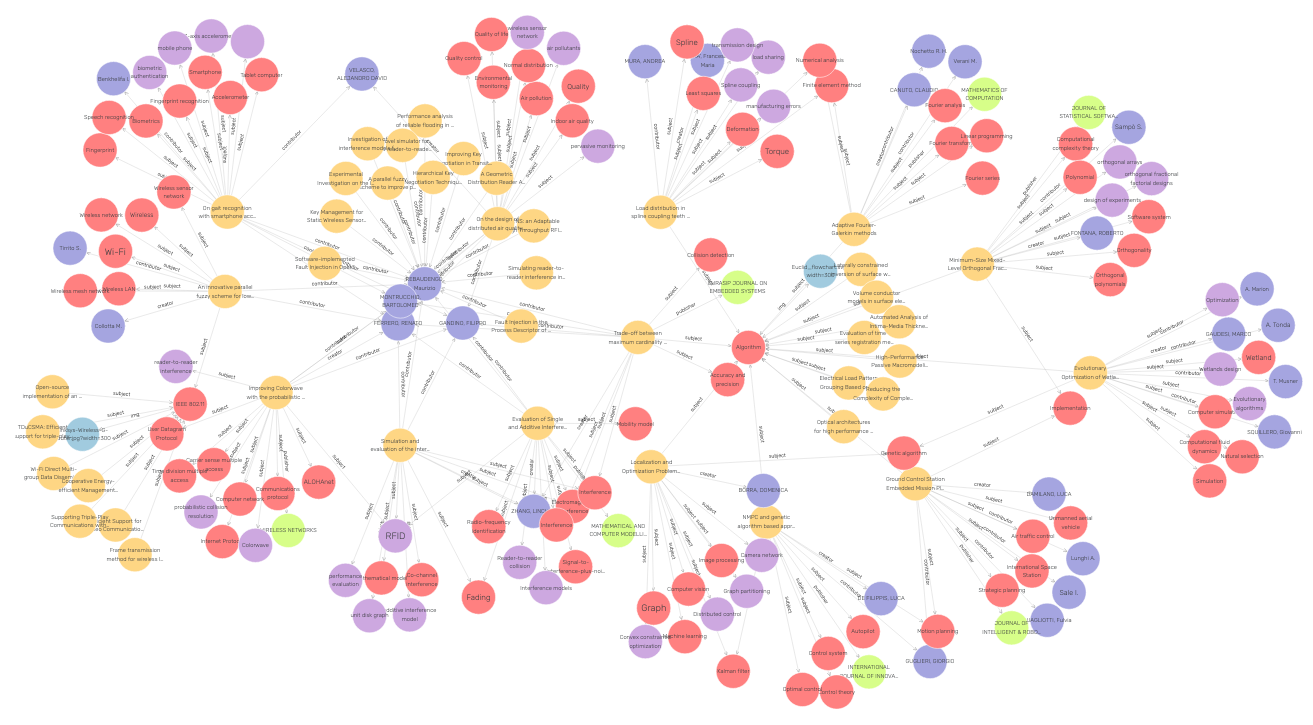
\includegraphics[scale=0.4]{img/geranium-knowledge-base-example.png}
    \caption{An extract of the Polito Knowledge Graph that will be introduced and
    described in the following chapters.}
    \label{fig:geranium-knowledge-base-example}
\end{figure}

If all the requirements and cautions are met, a well formed knowledge base may
prove to be a critical resource for an organization. It allows not only to
build new services upon it, but also to improve the existing knowledge inside
the organization by performing reasoning upon the available knowledge, thus
to discover implicit facts that can be derived from existing relationships.
Another field of applications is the development of Expert Systems, AI
software that emulates the behavior of a human decision-making process by
navigating the knowledge base and taking decisions like in a rule-based system.

Today's knowledge bases are commonly composed by tens of
thousands nodes and by hundreds of thousands of edges, such giant data
structures pose many challenges.
Not only storing and querying giant graphs requires the adoption of
specialized DBMS that are capable of efficiently store and query the RDF
input representation, but also doing analysis and gathering statistics from
such giant graphs requires the adoption of highly efficient algorithms in
order to retrieve the desired output in an acceptable time.

The availability of such a complex and informative data structure leads
to the opening of interesting scenarios, especially when thinking about
the latent information that can be extracted from it. In
fact, a knowledge base is a structured representation of the
human knowledge in a specific field, thus its comprehensiveness is restricted
by the human understanding.


\section{Learning on Graphs}

\subsection{Representation learning}

Machine learning (ML) algorithms are used to learn models from the
available data, with the final goal to obtain a set of parameters
that are fine-tuned to identify seen characteristics in the data
used for training. The models obtained can be later used to
recognize unseen inputs by leveraging the knowledge embedded
in such parameters.
ML algorithms require the input data to be available in a
machine-understandable vector representation. An important task
in the ML field is the learning of such representations, task known
as representation learning.

Natural Language Processing (NLP) is one of the research branches that in
the past years has made a great use of machine learning algorithms both for
language recognition and for embedding words \emph{meaning} into words
\emph{vectors}.
One of the most successful algorithms when dealing with representation learning
of words is Word2Vec \cite{mikolov2013}, where the model obtained is trained to
learn a vector representation for each word in a vocabulary.
In Word2Vec, the concept of meaning of a word is related to the context in
which such word is frequently used, so two words are recognized as similar if
they're used in similar contexts, thus in the vector space of the learnt
representations words that have similar meaning have higher cosine similarity
with respect to dissimilar ones.
For instance, the cosine similarity between the word vectors of "Man" and "King"
is roughly the same as the one between the words "Woman" and "Queen", since such
words are used in similar contexts. This has open up new scenarios for
language recognition and processing, since it allowed to perform vector
operations on such words which brought interesting results, as can be seen
in figure \ref{fig:word2vec}.

\begin{figure}[h]
    \centering
    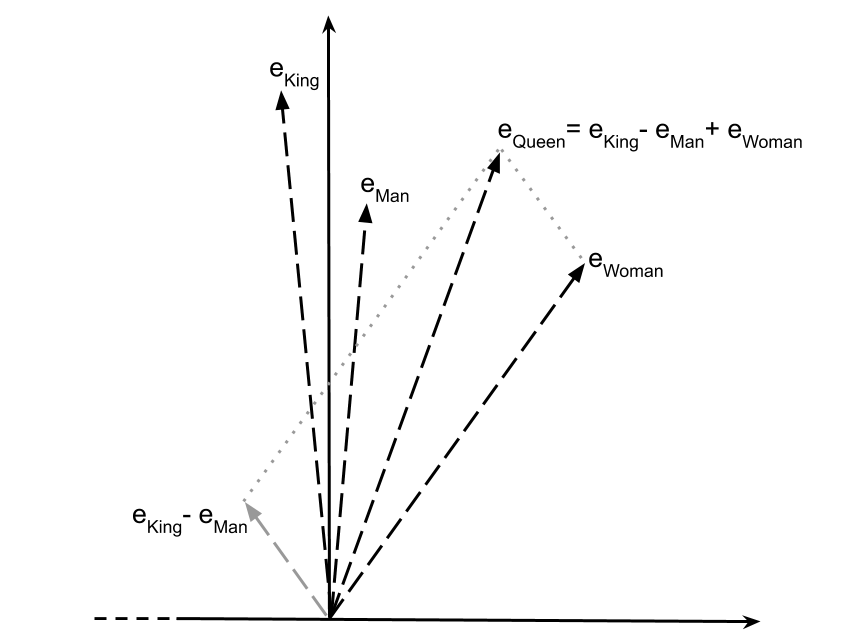
\includegraphics[scale=0.4]{img/word2vec.png}
    \caption{
        Word vectors allows to perform vector operations, the results
        obtained reflect the fact that Word2Vec is capable of embed the
        meaning of such words.
    }
    \label{fig:word2vec}
    \end{figure}

The idea that words can be characterized by the context in which they're used
can be generalized and used into other fields of research, such as
the field of representation learning on graphs.

Graphs are composed by nodes and edges, and are used to describe complex
systems, such as social networks or the interactions in a molecular biology
system. To apply machine learning algorithms to such data structures, in order
to analyze the available data and predict new facts, vector representations of
such nodes and edges are needed. Such vector representations are often
referred to as \emph{embeddings}.

Early approaches required these representations to be learned from feature
vectors that where handcrafted, task that required not
only a relevant amount of effort, but also a deep understanding of the domain
of interest. This has long been one of the main obstacles when dealing with
representation learning tasks, since who has knowledge of the domain and who
has to engineer the features were unlikely the same individual.


\subsection{Deep Learning on graphs}

In the latest years a big shift towards deep architectures has been made
in machine learning, mainly thanks to the development of highly
parallelized architectures that are able to efficiently compute
at the hardware level vector and matrix multiplications, operations that
are at the basis of any machine learning task.
Deep Learning (DL) algorithms are able to extract relevant features from
raw data by applying simple mathematical operations, such as convolution, to
the input data.
An example of one of the most successful applications of DL is in
image recognition, where matrix representations of images are
convolved with self-trained filters that are able to
extract the relevant features needed to recognize patterns present
in the input images.

Deep learning techniques have proven to function well also in the field of
representation learning for graph data, this should not give rise to surprise,
given that as can be seen in figure \ref{fig:pixels-as-graph}, a digital image
is composed by pixels which can be thought of as nodes in a graph, where
each pixel is connected by an edge to its immediate neighbors. This suggests
that the techniques used when dealing with images can be adapted, with
some major changes, to the field of representation learning on graphs, but
also in other fields of research, such as learning on manifolds.

\begin{figure}[h]
    \centering
    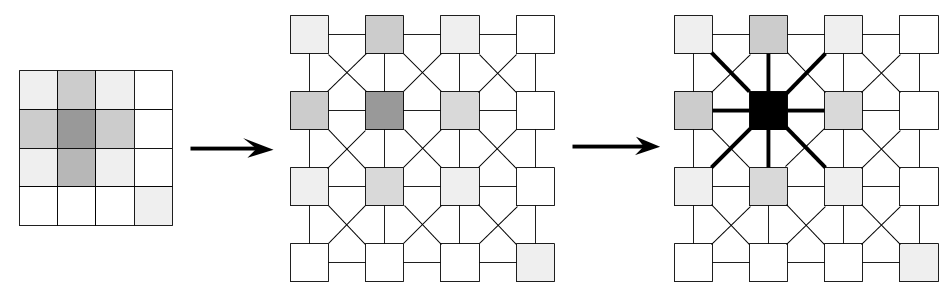
\includegraphics[scale=0.4]{img/pixels-as-graph.png}
    \caption{A digital image can be thought of as a graph.}
    \label{fig:pixels-as-graph}
\end{figure}

The problems when working with graph data is that commonly graphs
are built to describe complex systems, such as the knowledge of a
domain or field for knowledge graphs, and thus are composed of
a fairly high amount of nodes and edges. The matrices used to
store the graph structure can thus explode in dimensionality, so as
to became impractical as input data. Moreover, graphs aren't
regular structures with given shape and size, like a matrix of pixels
for images, but they live in an irregular domain which led to highly
irregular structures.
The first problem can be solved by randomly sampling the graph at each
training epoch, the immediate drawback being that more than one epoch
is required to train over all nodes. The second problem can instead be
solved by adapting known algorithms to work on highly irregular domains.
One of the possible approaches, which has proven to work well, is
the one based on convolutions.

Graph Convolutional Networks (GCNs) \cite{kipf2016} are a class of
semi-supervised deep learning algorithms for graphs which are based on the
same convolution and backpropagation operations as the so famous
Convolutional Neural Networks (CNNs) used for feature learning on
images.
The main difference between CNNs and GCNs is in the architecture of
the neural network, and so in how the convolution is performed, instead
the backpropagation phase is the same as the one used to update the
parameters of CNNs, with the loss function being task-specific.
In a CNN the input matrix of each network layer, which is the pixel matrix
of the input image for the first layer, is convolved with a convolutional
filter, whose parameters are then updated during the backpropagation phase.

GCNs works differently, but similarly, by convolving at the l-th layer
of the network the feature vector of each node with the feature
vectors of its l-nearest neighbors, this is done by applying the following
transformation:

\begin{equation}
H^{l+1}=\sigma(\tilde{D}^{-1/2}\tilde{A}\tilde{D}^{-1/2}H^lW^l)
\end{equation}

Where $H^{l}$ is the output of the previous layer or, for the input layer, the
nodes feature matrix where each row is commonly initialized
as a one-hot encoded feature vector. $\tilde{A}$ is the adjacency matrix
of the graph summed with the identity matrix to add self loops of nodes,
$\tilde{D}$ is the node degree matrix of $\tilde{A}$ and is used to
normalize it, $W^l$ is the weight matrix of the layer, that is shared
among all nodes for each layer, just like the convolutional filter in a CNN,
and $\sigma()$ is a non linear activation function, like $ReLU$.

Analyzing the forward rule for a single node make it more clear how the
embedding of a node is updated through the convolution:

\begin{equation}
    h^{(l+1)}_{i}=\sigma(\sum_{j\in\eta_{i}} \frac{1}{c_{ij}}h_j^{(l)}W^{{(l)}})
\end{equation}

Setting aside the normalization costant $c_{ij}$ which is obtained from the
multiplication between the adjancency and degree matrices, at each layer the
updated feature vector of the node $i$ is obtained by summing over all the
nodes in its neighborhood the result of the multiplication between the
neighbors feature vectors and the weight matrix of the layer.
A consequences of applying this rule to all nodes is that at the l-th layer
the feature vectors of nodes that are at a $l$ hop distance from the node $i$
will be embedded in its feature vector, because the feature vectors of such
nodes were embedded, at the previous layer, by the immediate neighbors of
node $i$, which are now passing the information of their surrounding to it.
So the amount of layers of the network is a parameter that controls how much
information for furthest nodes has to be collected from each node embedding.

\begin{figure}[h]
    \centering
    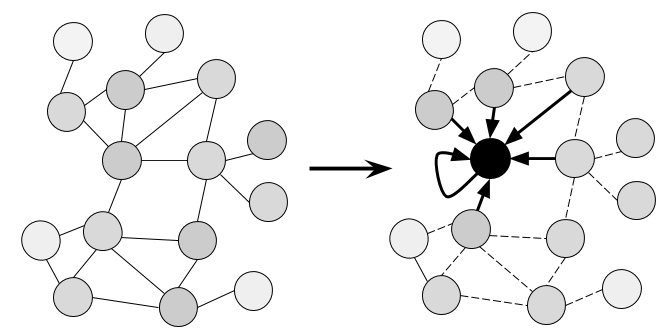
\includegraphics[scale=0.4]{img/gcn.png}
    \caption{First layer of a GCN updating a node feature vector by embedding
        the features of adjacent nodes.}
    \label{fig:gcn}
\end{figure}

This means that each node embedding will be characterized by its context,
just like it happens in Word2Vec, but in a non-Euclidean domain.
So for example, in a social graph where each person is characterized by its
friends, interests, places visited and so on, two people will have similar
embeddings if they are connected to similar nodes.

The node embeddings obtained by applying a GCN or one of its variants can
then be used to perform some learning task on the graph, like classification
of unseen nodes or link prediction of non-existent edges, the latter being
one of the most interesting task because it empowers most of the
recommendation systems available in the industry.



\chapter{State of the art}










\chapter{Approach and Methodology}

\chapter{Development and Implementation}

\chapter{Evaluation}

\chapter{Conclusions}


%%%%%%%%%%%%%%%%%%%%%%
% BEGIN bibliography %
%%%%%%%%%%%%%%%%%%%%%%
\bibliographystyle{IEEEtran}
\bibliography{references}

\end{document}
